%
% Modified by Megan Patnott
% Last Change: Jan 18, 2013
%
%%%%%%%%%%%%%%%%%%%%%%%%%%%%%%%%%%%%%%%%%%%%%%%%%%%%%%%%%%%%%%%%%%%%%%%%
%
% Modified by Sameer Vijay
% Last Change: Wed Jul 27 2005 13:00 CEST
%
%%%%%%%%%%%%%%%%%%%%%%%%%%%%%%%%%%%%%%%%%%%%%%%%%%%%%%%%%%%%%%%%%%%%%%%%
%
% Sample Notre Dame Thesis/Dissertation
% Using Donald Peterson's ndthesis classfile
%
% Written by Jeff Squyres and Don Peterson
%
% Provided by the Information Technology Committee of
%   the Graduate Student Union
%   http://www.gsu.nd.edu/
%
% Nothing in this document is serious except the format.  :-)
%
% If you have any suggestions, comments, questions, please send e-mail
% to: ndthesis@gsu.nd.edu
%
%%%%%%%%%%%%%%%%%%%%%%%%%%%%%%%%%%%%%%%%%%%%%%%%%%%%%%%%%%%%%%%%%%%%%%%%

%
% Chapter 4
%

\chapter{DIELECTRIC PROPERTIES}
\label{chap:dielectric}
In the chapter 3, I have presented various physical properties calculated using SP, GSF,TSF, and Ewald methods. This chapter reports on the fluctuation, perturbation, and potential of mean force (PMF) methods for calculating dielectric properties for dipolar and quadrupolar fluids. Since the dielectric constant is a macroscopic property, interactions of a molecule with the all of the molecules in the system should be considered. But the real space methods utilize a cutoff radius and ignores the interaction beyond cutoff radius. Hence the formula for calculating dielectric constant should be modified accordingly. To evaluate correct dielectric properties from the simulation, we have to take account of correction factor for each real-space methods. In this chapter, I have also presented the correction factor required for the calculation of the dielectric properties for dipolar and quadrupolar fluids.

\section{Introduction}

One of the most stringent tests of any new electrostatic method is the
fidelity with which that method can reproduce the bulk-phase
polarizability or equivalently, the dielectric properties of a
fluid. Before the advent of computer simulations, Kirkwood and Onsager
developed fluctuation formulae for the dielectric properties of
dipolar fluids.\cite{Kirkwood39,Onsagar36} Along with projections of
the frequency-dependent dielectric to zero frequency, these
fluctuation formulae are now widely used to predict the static
dielectric constant of simulated materials.

If we consider a system of dipolar or quadrupolar molecules under the
influence of an external field or field gradient, the net polarization
of the system will largely be proportional to the applied
perturbation.\cite{Chitanvis96, Stern-Feller03, SalvchovI14,SalvchovII14} In simulations, the net polarization of the system is
also determined by the interactions \textit{between} the
molecules. Therefore the macroscopic polarizablity obtained from a
simulation depends on the details of the electrostatic interaction
methods that were employed in the simulation. To determine the
relevant physical properties of the multipolar fluid from the system
fluctuations, the interactions between molecules must be incorporated
into the formalism for the bulk properties.

In most simulations, bulk materials are treated using periodic
replicas of small regions, and this level of approximation requires
corrections to the fluctuation formulae that were derived for the bulk
fluids. In 1983 Neumann proposed a general formula for evaluating
dielectric properties of dipolar fluids using both Ewald and
real-space cutoff methods.\cite{NeumannI83} Steinhauser and Neumann
used this formula to evaluate the corrected dielectric constant for
the Stockmayer fluid using two different methods: Ewald-Kornfeld (EK)
and reaction field (RF) methods.\cite{NeumannII83}

Zahn \textit{et al.}\cite{Zahn02} utilized this approach and evaluated
the correction factor for using damped shifted charge-charge
kernel. This was later generalized by Izvekov \textit{et
  al.},\cite{Izvekov08} who noted that the expression for the
dielectric constant reduces to widely-used conducting boundary formula
for real-space methods that have first derivatives that vanish at the
cutoff radius.

One of the primary topics of this chapter is the derivation of
correction factors for the three new real space methods.  We find that
the correction formulae for dipolar molecules depends not only on the
methodology being used, but also on whether the molecular dipoles are
treated using point charges or point dipoles.  We derive correction
factors for both cases.

In quadrupolar fluids, the relationship between quadrupolar
susceptibility and the dielectric constant is not as straightforward
as in the dipolar case.  The effective dielectric constant depends on
the geometry of the external (or internal) field
perturbation.\cite{Ernst92} Significant efforts have been made to
increase our understanding the dielectric properties of these
fluids,\cite{JeonI03,JeonII03,Chitanvis96} although a general
correction formula has not yet been developed.

In this chapter, we derive general formulae for calculating the
quadrupolar susceptibility of quadrupolar fluids. We also evaluate the
correction factor for SP, GSF, and TSF methods for quadrupolar fluids
interacting via point charges, point dipoles or directly through
quadrupole-quadrupole interactions.

We also calculate the screening behavior for two ions immersed in
multipolar fluids to estimate the distance dependence of charge
screening in both dipolar and quadrupolar fluids.  We use three
distinct methods to compare our analytical results with computer
simulations:
\begin{enumerate}
\item responses of the fluid to external perturbations,
\item fluctuations of system multipole moments, and
\item potentials of mean force between solvated ions,
\end{enumerate}

\begin{figure}
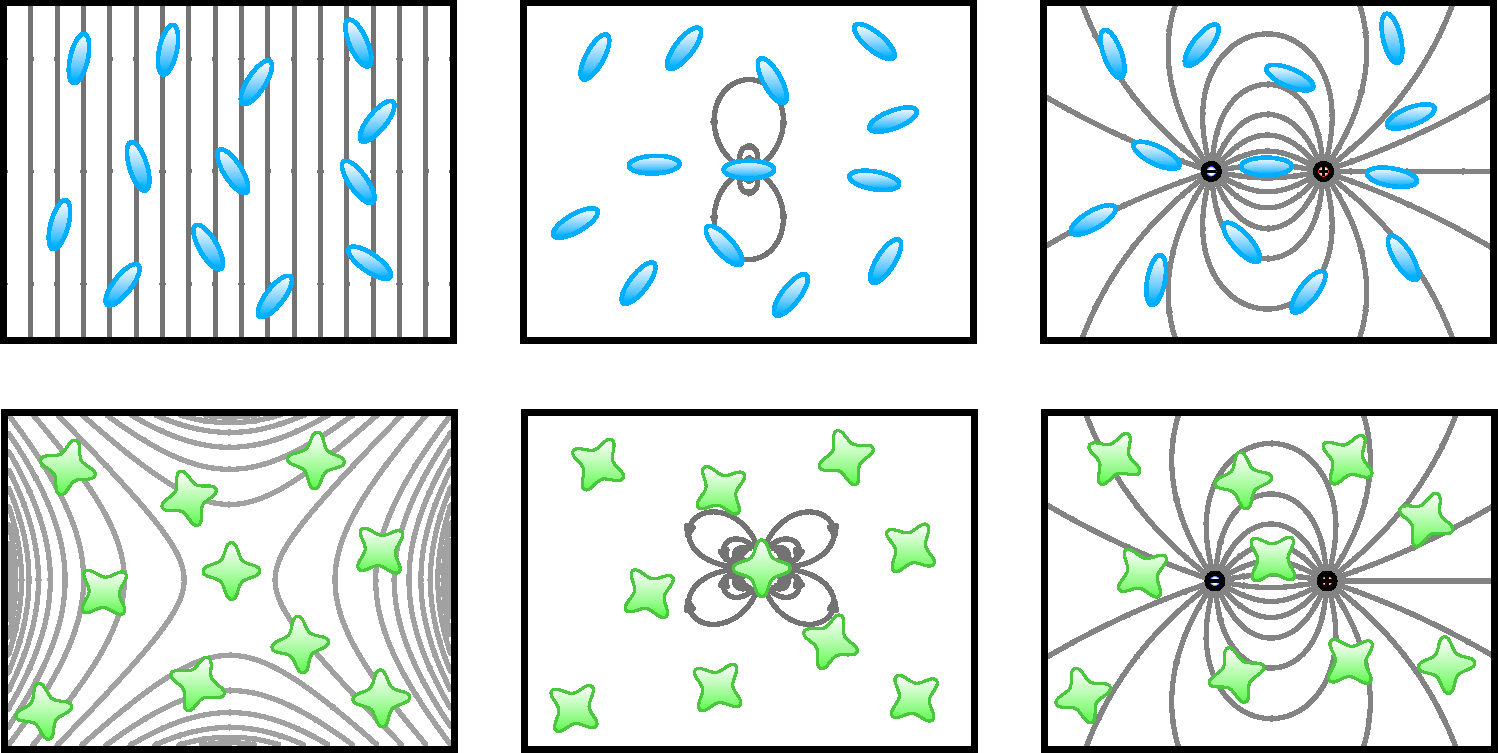
\includegraphics[width=\linewidth]{Schematic}
\caption{Dielectric properties of a fluid measure the response to
  external electric fields and gradients (left), or internal fields
  and gradients generated by the molecules themselves (center), or
  fields produced by embedded ions (right). The dielectric constant
  ($\epsilon$) measures all three responses in dipolar fluids (top).
  In quadrupolar liquids (bottom), the relevant bulk property is the
  quadrupolar susceptibility ($\chi_Q$), and the geometry of the field
  determines the effective dielectric screening.}
\label{fig:schematic}
\end{figure}

Under the influence of weak external fields, the bulk polarization of
the system is primarily a linear response to the perturbation, where
proportionality constant depends on the electrostatic interactions
between the multipoles. The fluctuation formulae connect bulk
properties of the fluid to equilibrium fluctuations in the system
multipolar moments during a simulation. These fluctuations also depend
on the form of the electrostatic interactions between molecules.
Therefore, the connections between the actual bulk properties and both
the computed fluctuation and external field responses must be modified
accordingly.

The potential of mean force (PMF) allows calculation of an effective
dielectric constant or screening factor from the potential energy
between ions before and after dielectric material is introduced.
Computing the PMF between embedded point charges is an additional
check on the bulk properties computed via the other two methods.

\section{Dipolar Fluids and the Dielectric Constant}

Dielectric properties of a fluid arise mainly from responses of the
fluid to either applied fields or transient fields internal to the
fluid. In response to an applied field, the molecules have electronic
polarizabilities, changes to internal bond lengths, and reorientations
towards the direction of the applied field. There is an added
complication that in the presence of external field, the perturbation
experienced by any single molecule is not only due to external field
but also to the fields produced by the all other molecules in the
system.

\subsection{Response to External Perturbations}

In the presence of uniform electric field $\mathbf{E}$, an individual
molecule with a permanent dipole moment $p_o$ will realign along the
direction of the field with an average polarization given by
\begin{equation}
\braket{\mathbf{p}} = \epsilon_0 \alpha_p \mathbf{E},
\end{equation}
where $\alpha_p = {p_o}^2 / 3 \epsilon_0 k_B T$ is the contribution to
molecular polarizability due solely to reorientation dynamics.
Because the applied field must overcome thermal motion, the
orientational polarization depends inversely on the temperature.

Likewise, a condensed phase system of permanent dipoles will also
polarize along the direction of an applied field. The polarization
density of the system is
\begin{equation}
\textbf{P} = \epsilon_o \alpha_{D} \mathbf{E}. 
\label{pertDipole}
\end{equation} 
The constant $\alpha_D$ is the macroscopic polarizability, which is an
emergent property of the dipolar fluid.  Note that the polarizability,
$\alpha_D$ is distinct from the dipole susceptibility, $\chi_D$,
which is the quantity most directly related to the static dielectric
constant, $\epsilon = 1 + \chi_D$.

\subsection{Fluctuation Formula}

For a system of dipolar molecules at thermal equilibrium, we can
define both a system dipole moment, $\mathbf{M} = \sum_i \mathbf{p}_i$
as well as a dipole polarization density,
$\mathbf{P} = \braket{\mathbf{M}}/V$.

In the presence of applied field $\mathbf{E}$, the polarization
density can be expressed in terms of fluctuations in the net dipole
moment,
\begin{equation}
\mathbf{P} = \epsilon_o \frac{\braket{\mathbf{M}^2}-{\braket{\mathbf{M}}}^2}{3 \epsilon_o V k_B T}\bf{E}
\label{flucDipole}
\end{equation}
This has structural similarity with the Boltzmann average for the
polarization of a single molecule. Here
$ \braket{\mathbf{M}^2}-{\braket{\mathbf{M}}}^2$ measures fluctuations
in the net dipole moment,
\begin{equation}
 \langle \mathbf{M}^2 \rangle - \langle \mathbf{M} \rangle^2 =
 \langle M_x^2+M_y^2+M_z^2 \rangle - \left( \langle M_x \rangle^2 +
   \langle M_y \rangle^2 +
   \langle M_z \rangle^2 \right).
\label{eq:flucDip}
\end{equation}
For the limiting case $\textbf{E} \rightarrow 0 $, the ensemble
average of both the net dipole moment $\braket{\mathbf{M}}$ and
dipolar polarization $\bf{P}$ tends to vanish but
$\braket{\mathbf{M}^2}$ does not.  The macroscopic dipole
polarizability can therefore be written as,
\begin{equation}
  \alpha_D = \frac{\braket{\mathbf{M}^2}-{\braket{\mathbf{M}}}^2}{3 \epsilon_o V k_B T}
\end{equation}
This relationship between a macroscopic property of dipolar material
and microscopic fluctuations is true even when the applied field
$ \textbf{E} \rightarrow 0 $.

\subsection{Correction Factors}
\label{sec:corrFactor}
In the presence of a uniform external field $ \mathbf{E}^\circ$, the
total electric field at $\mathbf{r}$ depends on the polarization
density at all other points in the system,\cite{NeumannI83}
\begin{equation}
\mathbf{E}(\mathbf{r}) = \mathbf{E}^\circ(\mathbf{r}) +
\frac{1}{4\pi\epsilon_o} \int d\mathbf{r}^\prime
\mathbf{T}(\mathbf{r}-\mathbf{r}^\prime)\cdot
{\mathbf{P}(\mathbf{r}^\prime)}.
\label{eq:localField}
\end{equation}
$\mathbf{T}$ is the dipole interaction tensor connecting dipoles at
$\mathbf{r}^\prime$ with the point of interest ($\mathbf{r}$).

In simulations of dipolar fluids, the molecular dipoles may be
represented either by closely-spaced point charges or by 
point dipoles (see Fig. \ref{fig:tensor}).
\begin{figure}
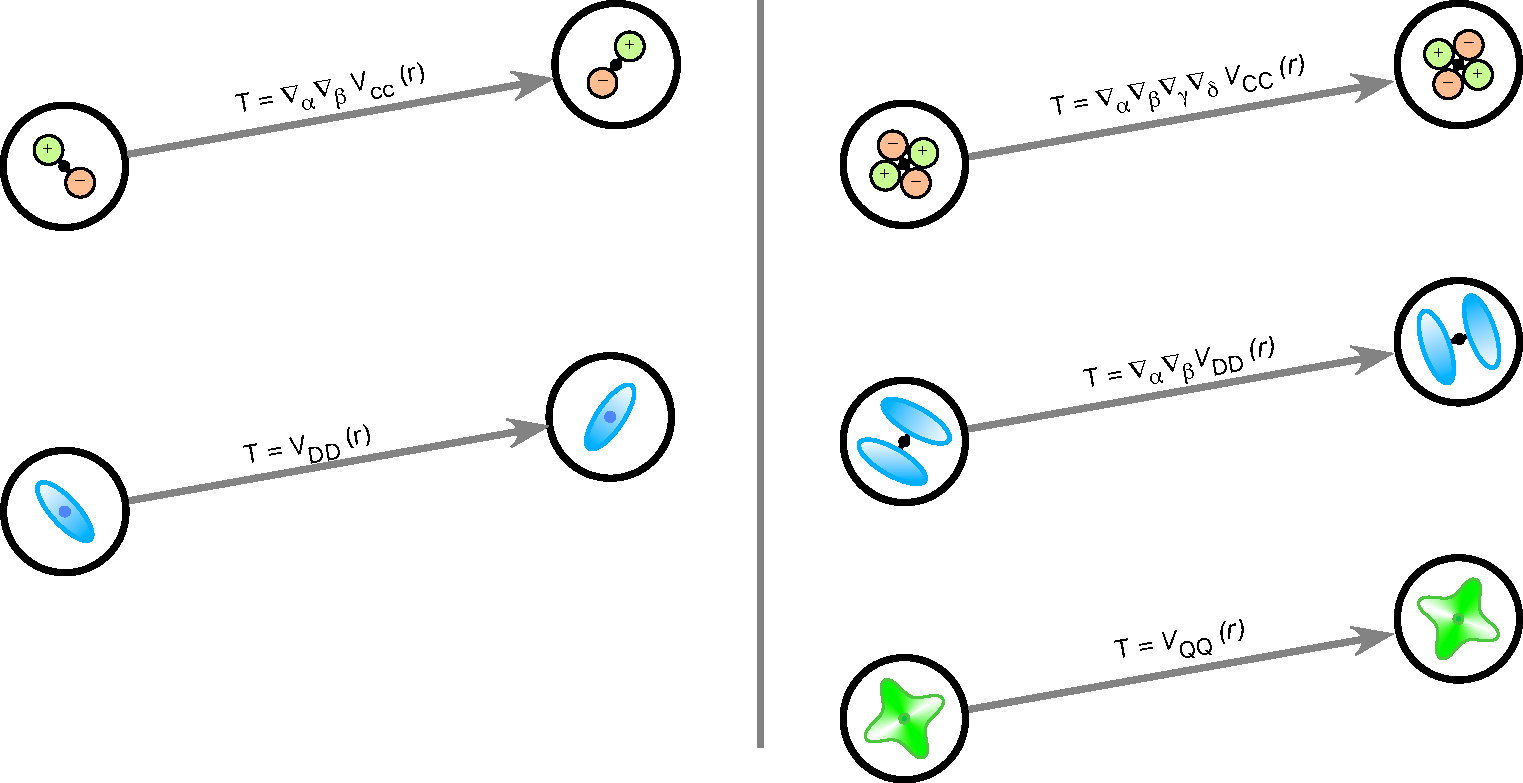
\includegraphics[width=\linewidth]{Tensors}
\caption{In the real-space electrostatic methods, the molecular dipole
  tensor, $\mathbf{T}_{\alpha\beta}(r)$, is not the same for
  charge-charge interactions as for point dipoles (left panel). The
  same holds true for the molecular quadrupole tensor (right panel),
  $\mathbf{T}_{\alpha\beta\gamma\delta}(r)$, which can have distinct
  forms if the molecule is represented by charges, dipoles, or point
  quadrupoles.}
\label{fig:tensor}
\end{figure}
In the case where point charges are interacting via an electrostatic
kernel, $v(r)$, the effective {\it molecular} dipole tensor,
$\mathbf{T}$ is obtained from two successive applications of the
gradient operator to the electrostatic kernel,
\begin{eqnarray}
\mathbf{T}_{\alpha \beta}(r) &=&  \nabla_\alpha \nabla_\beta
                               \left(v(r)\right)  \\
  &=& \delta_{\alpha \beta}
\left(\frac{1}{r} v^\prime(r) \right) + \frac{r_{\alpha}
  r_{\beta}}{r^2} \left( v^{\prime \prime}(r) - \frac{1}{r}
  v^{\prime}(r) \right)
\label{dipole-chargeTensor}
\end{eqnarray}
where $v(r)$ may be either the bare kernel ($1/r$) or one of the
modified (Wolf or DSF) kernels.  This tensor describes the effective
interaction between molecular dipoles ($\mathbf{D}$) in Gaussian units
as $-\mathbf{D} \cdot \mathbf{T} \cdot \mathbf{D}$.

When utilizing any of the three new real-space methods for point
\textit{dipoles}, the tensor is explicitly constructed,
\begin{equation}
\mathbf{T}_{\alpha \beta}(r)  =  \delta_{\alpha \beta} v_{21}(r) +
\frac{r_{\alpha} r_{\beta}}{r^2} v_{22}(r) 
\label{dipole-diopleTensor}
\end{equation}
where the functions $v_{21}(r)$ and $v_{22}(r)$ depend on the level of
the approximation.\cite{PaperI,PaperII} Although the Taylor-shifted
(TSF) and gradient-shifted (GSF) models produce to the same $v(r)$
function for point charges, they have distinct forms for the
dipole-dipole interaction.
 
Using a constitutive relation, the polarization density
$\mathbf{P}(\mathbf{r})$ is given by,
\begin{equation}
\mathbf{P}(\mathbf{r}) = \epsilon_o \chi_D
\left(\mathbf{E}^\circ(\mathbf{r}) + \frac{1}{4\pi\epsilon_o} \int
  d\mathbf{r}^\prime \mathbf{T}(\mathbf{r}-\mathbf{r}^\prime ) \cdot \mathbf{P}(\mathbf{r}^\prime)\right).
\label{constDipole}
\end{equation}
Note that $\chi_D$ explicitly depends on the details of the dipole
interaction tensor.  Neumann \textit{et al.}
\cite{NeumannI83,NeumannII83,Neumann84,Neumann85} derived an elegant
way to modify the fluctuation formula to correct for approximate
interaction tensors. This correction was derived using a Fourier
representation of the interaction tensor,
$\tilde{\mathbf{T}}(\mathbf{k})$, and involves the quantity,
\begin{equation}
 A = \frac{3}{4\pi}\tilde{\mathbf{T}}(0) = \frac{3}{4\pi} \int_V
 d\mathbf{r} \mathbf{T}(\mathbf{r})
 \label{dipCorrFactor}
\end{equation}
which is the $k \rightarrow 0$ limit of $\tilde{\mathbf{T}}$.  Using
this quantity (originally called $Q$ in
Refs.~\cite{NeumannI83,NeumannII83,Neumann84,Neumann85}), the
dielectric constant can be computed
\begin{equation}
\epsilon = \frac{3+(A + 2)(\epsilon_{CB}-1)}{3 + (A -1)(\epsilon_{CB}-1)}
\label{correctionFormula}
\end{equation}
where $\epsilon_{CB}$ is the widely-used conducting boundary
expression for the dielectric constant,
\begin{equation}
\epsilon_{CB} = 1 + \frac{\braket{\bf{M}^2}-{\braket{\bf{M}}}^2}{3
  \epsilon_o V k_B T} = 1 + \alpha_{D}
\label{conductingBoundary}
\end{equation}
Eqs.~(\ref{correctionFormula}) and (\ref{conductingBoundary}) allows
estimation of the static dielectric constant from fluctuations easily
computed directly from simulations.

We have utilized the Neumann \textit{et al.} approach for the three
new real-space methods, and obtain method-dependent correction
factors.  The expression for the correction factor also depends on
whether the simulation involves point charges or point dipoles to
represent the molecular dipoles.  These corrections factors are 
listed in Table~\ref{tab:A}. We note that the GSF correction factor for
point dipoles has been independently derived by Stenqvist \textit{et
  al.}\cite{Stenqvist:2015ph}

\begin{sidewaystable}[tpb]
	\begin{center}
  	\caption{Expressions for the dipolar correction factor ($A$) for the
    real-space electrostatic methods in terms of the damping parameter 
    ($\alpha$) and the cutoff radius ($r_c$).  The Ewald-Kornfeld result 
    derived in Refs.\cite{Adams80,Adams81,NeumannI83} is shown
    for comparison using the Ewald convergence parameter ($\kappa$)
    and the real-space cutoff value ($r_c$). } 
		\label{tab:A}
	\begin{tabular}{l|c|c}
	%\toprule
	\hline       
	& \multicolumn{2}{c}{Molecular Representation} \\ 
	Method & point charges & point dipoles  \\ \hline
	\colrule
 		Shifted Potental (SP) & $ \mathrm{erf}(r_c \alpha) - \frac{2
                               \alpha r_c}{\sqrt{\pi}} e^{-\alpha^2
                               r_c^2}$ & $\mathrm{erf}(r_c \alpha)
                                         -\frac{2 \alpha
                                         r_c}{\sqrt{\pi}}\left(1+\frac{2\alpha^2
                                         {r_c}^2}{3}
                                         \right)e^{-\alpha^2{r_c}^2}
                                         $\\ \colrule
	Gradient-shifted  (GSF) & 1 & $\mathrm{erf}(\alpha  r_c)-\frac{2
                              \alpha  r_c}{\sqrt{\pi}}  \left(1 +
                              \frac{2 \alpha^2 r_c^2}{3} +
                              \frac{\alpha^4
                              r_c^4}{3}\right)e^{-\alpha^2 r_c^2} $ \\ \colrule
	Taylor-shifted  (TSF) & 1 & 1  \\ \colrule
	Spherical Cutoff (SC)& $\mathrm{erf}(r_c \alpha) -
                        \frac{2 \alpha r_c}{\sqrt{\pi}} e^{-\alpha^2
                        r_c^2}$ & $\mathrm{erf}(r_c \alpha) -
                        \frac{2 \alpha r_c}{\sqrt{\pi}} e^{-\alpha^2
                        r_c^2}$ \\ 
	Ewald-Kornfeld (EK) & $\mathrm{erf}(r_c \kappa) -
                      \frac{2 \kappa r_c}{\sqrt{\pi}} e^{-\kappa^2
                      r_c^2}$ & $\mathrm{erf}(r_c \kappa) -
                      \frac{2 \kappa r_c}{\sqrt{\pi}} e^{-\kappa^2
                      r_c^2}$  \\ \hline
%\botrule
	\end{tabular}
	\end{center}
\end{sidewaystable}
Note that for point charges, the GSF and TSF methods produce estimates
of the dielectric that need no correction, and the TSF method likewise
needs no correction for point dipoles. 

\section{Quadrupolar Fluids and the Quadrupolar Susceptibility}
\subsection{Response to External Perturbations}

A molecule with a permanent quadrupole, $\mathsf{q}$, will align in
the presence of an electric field gradient $\nabla\mathbf{E}$.  The
anisotropic polarization of the quadrupole is given
by,\cite{AduGyamfi78,AduGyamfi81}
\begin{equation}
\braket{\mathsf{q}} - \frac{\mathbf{I}}{3}
\mathrm{Tr}(\mathsf{q}) = \epsilon_o \alpha_q \nabla\mathbf{E},
\end{equation}
where $\alpha_q = q_o^2 / 15 \epsilon_o k_B T $ is a molecular quadrupole
polarizablity and $q_o$ is an effective quadrupole moment for the molecule,
\begin{equation}
 q_o^2 = 3 \mathsf{q}:\mathsf{q} - \mathrm{Tr}(\mathsf{q})^2.
\end{equation}

In the presence of an external field gradient, a system of quadrupolar
molecules also organizes with an anisotropic polarization,
\begin{equation}
\mathsf{Q} - \frac{\mathbf{I}}{3} \mathrm{Tr}(\mathsf{Q}) =  \epsilon_o
\alpha_Q  \nabla\mathbf{E}
\end{equation}
where $\mathsf{Q}$ is the traced quadrupole density of the system and
$\alpha_Q$ is a macroscopic quadrupole polarizability which has
dimensions of $\mathrm{length}^{-2}$. Equivalently, the traceless form
may be used,
\begin{equation}
\mathsf{\Theta} = 3 \epsilon_o  \alpha_Q \nabla\mathbf{E},
\label{pertQuad}
\end{equation} 
where
$\mathsf{\Theta} = 3\mathsf{Q} - \mathbf{I} \mathrm{Tr}(\mathsf{Q})$
is the traceless tensor that also describes the system quadrupole
density.  It is this tensor that will be utilized to derive correction
factors below.

\subsection{Fluctuation Formula}
As in the dipolar case, we may define a system quadrupole moment,
$\mathsf{M}_Q = \sum_i \mathsf{q}_i$ and the traced quadrupolar
density, $\mathsf{Q} = \mathsf{M}_Q / V$.  A fluctuation formula can
be written for a system comprising quadrupolar
molecules,\cite{LoganI81,LoganII82,LoganIII82}
\begin{equation}
\mathsf{Q} - \frac{\mathbf{I}}{3} \mathrm{Tr}(\mathsf{Q}) = \epsilon_o
\frac{\braket{\mathsf{M}_Q^2}-{\braket{\mathsf{M}_Q}}^2}{15 \epsilon_o
  V k_B T} \nabla\mathbf{E}.
\label{flucQuad}
\end{equation}
Some care is needed in the definitions of the averaged quantities.  These
refer to the effective quadrupole moment of the system, and they are
computed as follows,
\begin{align}
\braket{\mathsf{M}_Q^2} &= \braket{3 \mathsf{M}_Q:\mathsf{M}_Q -
  \mathrm{Tr}(\mathsf{M}_Q)^2 }\\
\braket{\mathsf{M}_Q}^2 &= 3 \braket{\mathsf{M}_Q}:\braket{\mathsf{M}_Q} -
\mathrm{Tr}(\braket{\mathsf{M}_Q})^2
\label{eq:flucQuad}
\end{align}
The macroscopic quadrupolarizability is given by,
\begin{equation}
  \alpha_Q = \frac{\braket{\mathsf{M}_Q^2}-{\braket{\mathsf{M}_Q}}^2}{15 \epsilon_o V k_B T}
\label{propConstQuad}
\end{equation}
This relationship between a macroscopic property of a quadrupolar
fluid and microscopic fluctuations should be true even when the
applied field gradient $\nabla \mathbf{E} \rightarrow 0$.

\subsection{Correction Factors}
In this section we generalize the treatment of Neumann \textit{et al.}
for quadrupolar fluids. Interactions involving multiple quadrupoles
are rank 4 tensors, and we therefore describe quantities in this
section using Einstein notation.

In the presence of a uniform external field gradient,
$\partial_\alpha {E}^\circ_\beta $, the total field gradient at
$\mathbf{r}$ depends on the quadrupole polarization density at all
other points in the system,
\begin{equation}
\partial_\alpha E_\beta(\mathbf{r}) = \partial_\alpha
{E}^\circ_\beta(\mathbf{r}) + \frac{1}{8\pi \epsilon_o}\int
T_{\alpha\beta\gamma\delta}({\mathbf{r}-\mathbf{r}^\prime})
Q_{\gamma\delta}(\mathbf{r}^\prime) d\mathbf{r}^\prime 
\label{gradMaxwell}
\end{equation}
where and $T_{\alpha\beta\gamma\delta}$ is the quadrupole interaction
tensor connecting quadrupoles at $\mathbf{r}^\prime$ with the point of
interest ($\mathbf{r}$).

In simulations of quadrupolar fluids, the molecular quadrupoles may be
represented by closely-spaced point charges, by multiple point
dipoles, or by a single point quadrupole (see
Fig. \ref{fig:tensor}).  In the case where point charges are
interacting via an electrostatic kernel, $v(r)$, the effective
molecular quadrupole tensor can obtained from four successive
applications of the gradient operator to the electrostatic kernel,
\begin{eqnarray}
T_{\alpha\beta\gamma\delta}(\mathbf{r}) &=& \nabla_\alpha \nabla_\beta
                                   \nabla_\gamma \nabla_\delta v(r) \\
 &=& \left(\delta_{\alpha\beta}\delta_{\gamma\delta} +
     \delta_{\alpha\gamma}\delta_{\beta\delta}+
     \delta_{\alpha\delta}\delta_{\beta\gamma}\right)\left(-\frac{v^\prime(r)}{r^3}
     + \frac{v^{\prime \prime}(r)}{r^2}\right) \nonumber \\
 & &+ \left(\delta_{\alpha\beta} r_\gamma r_\delta + 5  \mathrm{~permutations}
     \right) \left(\frac{3v^\prime(r)}{r^5}-\frac{3v^{\prime \prime}(r)}{r^4} +
     \frac{v^{\prime \prime \prime}(r)}{r^3}\right) \nonumber \\
 & &+ r_\alpha r_\beta r_\gamma r_\delta
     \left(-\frac{15v^\prime(r)}{r^7}+\frac{15v^{\prime \prime}(r)}{r^6}-\frac{6v^{\prime
     \prime \prime}(r)}{r^5} + \frac{v^{\prime \prime \prime \prime}(r)}{r^4}\right),
\label{quadCharge}
\end{eqnarray}
where $v(r)$ can either be the electrostatic kernel ($1/r$) or one of
the modified (Wolf or DSF) kernels.  

Similarly, when representing quadrupolar molecules with multiple point
\textit{dipoles}, the molecular quadrupole interaction tensor can be
obtained using two successive applications of the gradient operator to
the dipole interaction tensor,
\begin{eqnarray}
T_{\alpha\beta\gamma\delta}(\mathbf{r}) &=& \nabla_\alpha \nabla_\beta
                                            T_{\gamma\delta}(\mathbf{r}) \\ 
& = & \delta_{\alpha\beta}\delta_{\gamma\delta} \frac{v^\prime_{21}(r)}{r} +
      \left(\delta_{\alpha\gamma}\delta_{\beta\delta}+
      \delta_{\alpha\delta}\delta_{\beta\gamma}\right)\frac{v_{22}(r)}{r^2}
      \nonumber\\ 
 & &+ \delta_{\gamma\delta} r_\alpha r_\beta
     \left(\frac{v^{\prime \prime}_{21}(r)}{r^2}-\frac{v^\prime_{21}(r)}{r^3} \right)\nonumber \\
 & &+\left(\delta_{\alpha\beta} r_\gamma r_\delta +
     \delta_{\alpha\gamma} r_\beta r_\delta  +\delta_{\alpha\delta}
     r_\gamma r_\beta + \delta_{\beta\gamma} r_\alpha r_\delta
     +\delta_{\beta\delta} r_\alpha r_\gamma  \right)
     \left(\frac{v^\prime_{22}(r)}{r^3}-\frac{2v_{22}(r)}{r^4}\right)
     \nonumber \\
 & &+ r_\alpha r_\beta r_\gamma r_\delta
     \left(\frac{v^{\prime
     \prime}_{22}(r)}{r^4}-\frac{5v^\prime_{22}(r)}{r^5}+\frac{8v_{22}(r)}{r^6}\right),
\label{quadDip}
\end{eqnarray}
where $T_{\gamma\delta}(\mathbf{r})$ is a dipole-dipole interaction
tensor that depends on the level of the
approximation.\cite{PaperI,PaperII} Similarly $v_{21}(r)$ and
$v_{22}(r)$ are the radial function for different real space cutoff
methods defined in the Chapter 2.\cite{PaperI}

For quadrupolar liquids modeled using point quadrupoles, the
interaction tensor can be constructed as,
\begin{eqnarray}
T_{\alpha\beta\gamma\delta}(\mathbf{r}) &=&
                                              \left(\delta_{\alpha\beta}\delta_{\gamma\delta}
                                              +
                                              \delta_{\alpha\gamma}\delta_{\beta\delta}+
                                              \delta_{\alpha\delta}\delta_{\beta\gamma}\right)v_{41}(r)
                                              + (\delta_{\gamma\delta} r_\alpha r_\beta +  \mathrm{ 5\; permutations}) \frac{v_{42}(r)}{r^2} \nonumber \\  
& & + r_\alpha r_\beta r_\gamma r_\delta  \left(\frac{v_{43}(r)}{r^4}\right), 
\label{quadRadial}
\end{eqnarray}
where again $v_{41}(r)$, $v_{42}(r)$, and $v_{43}(r)$ are radial
functions defined in Chapter 2. \cite{PaperI} Note that
these radial functions have different functional forms depending on
the level of approximation being employed.

The integral in Eq.~(\ref{gradMaxwell}) can be divided into two
parts, $|\mathbf{r}-\mathbf{r}^\prime|\rightarrow 0 $ and
$|\mathbf{r}-\mathbf{r}^\prime|> 0$. Since the self-contribution to
the field gradient vanishes at the singularity (see the supporting
information), Eq.~(\ref{gradMaxwell}) can be written as,
\begin{equation}
\partial_\alpha E_\beta(\mathbf{r}) = \partial_\alpha {E}^\circ_\beta(\mathbf{r}) +
  \frac{1}{8\pi \epsilon_o}\int\limits_{|\mathbf{r}-\mathbf{r}^\prime|> 0 }
  T_{\alpha\beta\gamma\delta}(\mathbf{r}-\mathbf{r}^\prime)
  {Q}_{\gamma\delta}(\mathbf{r}^\prime) d\mathbf{r}^\prime.
\end{equation}
If $\mathbf{r} = \mathbf{r}^\prime$ is excluded from the integration,
the total gradient can be most easily expressed in terms of
traceless quadrupole density as below,\cite{LoganI81}
\begin{equation}
\partial_\alpha E_\beta(\mathbf{r}) = \partial_\alpha
{E}^\circ_\beta(\mathbf{r}) + \frac{1}{24\pi
  \epsilon_o}\int\limits_{|\mathbf{r}-\mathbf{r}^\prime|> 0 }
T_{\alpha\beta\gamma\delta}(\mathbf{r}-\mathbf{r}^\prime) \Theta_{\gamma\delta}(\mathbf{r}') d\mathbf{r}^\prime,
\end{equation}
where
$\Theta_{\alpha\beta} = 3Q_{\alpha\beta} - \delta_{\alpha\beta}Tr(Q)$
is the traceless quadrupole density. In analogy to
Eq.~(\ref{pertQuad}) above, the quadrupole polarization density may
now be related to the quadrupolar susceptibility, $\chi_Q$,
\begin{equation}
\frac{1}{3}{\Theta}_{\alpha\beta}(\mathbf{r}) = \epsilon_o {\chi}_Q
\left[\partial_\alpha {E}^\circ_\beta(\mathbf{r}) + \frac{1}{24\pi
    \epsilon_o}\int\limits_{|\mathbf{r}-\mathbf{r}^\prime|> 0 }
  T_{\alpha\beta\gamma\delta}(\mathbf{r}-\mathbf{r}^\prime)
  \Theta_{\gamma\delta}(\mathbf{r}^\prime) d\mathbf{r}^\prime \right].
\end{equation}
For periodic boundaries and with a uniform imposed
$\partial_\alpha E^\circ_\beta$, the quadrupole density
${\Theta}_{\alpha\beta}$ will be uniform over the entire space. After
performing a Fourier transform (see the Appendix in
Ref.\cite{NeumannI83}) we obtain,
\begin{equation}
\frac{1}{3}\tilde{\Theta}_{\alpha\beta}(\mathbf{k})=
\epsilon_o {\chi}_Q \left[{\partial_\alpha
    \tilde{E}^\circ_\beta}(\mathbf{k})+ \frac{1}{24\pi
    \epsilon_o} \tilde{T}_{\alpha\beta\gamma\delta}(\mathbf{k})
 \tilde{\Theta}_{\gamma\delta}(\mathbf{k})\right].
\label{fourierQuad}
\end{equation} 
If the applied field gradient is homogeneous over the entire volume,
${\partial_ \alpha \tilde{E}^\circ_\beta}(\mathbf{k}) = 0 $ except at
$ \mathbf{k} = 0$. Similarly, the quadrupolar polarization density can
also considered uniform over entire space. As in the dipolar case,
\cite{NeumannI83} the only relevant contribution from the interaction
tensor will also be when $\mathbf{k} = 0$. Therefore Eq.~(\ref{fourierQuad}) can be written as,
\begin{equation}
\frac{1}{3}\tilde{\Theta}_{\alpha\beta}(\mathrm{0})=
\epsilon_o {\chi}_Q \left[{\partial_\alpha
    \tilde{E}^\circ_\beta}(\mathrm{0})+ \frac{1}{24\pi
    \epsilon_o} \tilde{T}_{\alpha\beta\gamma\delta}(\mathrm{0})
 \tilde{\Theta}_{\gamma\delta}(\mathrm{0})\right].
\label{fourierQuadZeroK}
\end{equation} 
The quadrupolar tensor
$\tilde{T}_{\alpha\beta\gamma\delta}(\mathrm{0})$ is a rank 4 tensor
with 81 elements. The only non-zero elements, however, are those with
two doubly-repeated indices, \textit{i.e.}
$\tilde{T}_{aabb}(\mathrm{0})$ and all permutations of these indices.
The special case of quadruply-repeated indices,
$\tilde{T}_{aaaa}(\mathrm{0})$ also survives (see appendix
\ref{ap:quadContraction}). Furthermore, for the both diagonal and
non-diagonal components of the quadrupolar polarization
$\tilde{\Theta}_{\alpha\beta}$, we can contract the second term in
Eq.~\ref{fourierQuadZeroK} (see appendix
\ref{ap:quadContraction}):
\begin{equation}
\tilde{T}_{\alpha\beta\gamma\delta}(\mathrm{0})\tilde{\Theta}_{\gamma\delta}(\mathrm{0})=
8 \pi \mathrm{B} \tilde{\Theta}_{\alpha\beta}(\mathrm{0}).
\label{quadContraction}
\end{equation}
Here $\mathrm{B} = \tilde{T}_{abab}(\mathrm{0}) / 4 \pi$ for
$a \neq b$.  Using this quadrupolar contraction we can solve Eq.~(\ref{fourierQuadZeroK}) as follows
\begin{eqnarray}
\frac{1}{3}\tilde{\Theta}_{\alpha\beta}(\mathrm{0}) &=& \epsilon_o
                                                      {\chi}_Q
                                                      \left[{\partial_\alpha
                                                      \tilde{E}^\circ_\beta}(\mathrm{0})+
                                                      \frac{\mathrm{B}}{3
                                                      \epsilon_o} 
                                                      {\tilde{\Theta}}_{\alpha\beta}(\mathrm{0})\right]
                                                      \nonumber \\                                                    
&=& \left[\frac{\epsilon_o {\chi}_Q} {1-{\chi}_Q \mathrm{B}}\right]
{\partial_\alpha \tilde{E}^\circ_\beta}(\mathrm{0}).
\label{fourierQuad2}
\end{eqnarray}
In real space, the correction factor is found to be,
\begin{equation}
\mathrm{B} = \frac{1}{4 \pi} \tilde{T}_{abab}(0) = \frac{1}{4 \pi} \int_V {T}_{abab}(\mathbf{r}) d\mathbf{r},
\end{equation}

which has been integrated over the interaction volume $V$ and has
units of $\mathrm{length}^{-2}$.

In terms of the traced quadrupole moment, Eq.~(\ref{fourierQuad2})
can be written,
\begin{equation}
\mathsf{Q} - \frac{\mathbf{I}}{3} \mathrm{Tr}(\mathsf{Q})
= \frac{\epsilon_o {\chi}_Q}{1-  {\chi}_Q \mathrm{B}} \nabla \mathbf{E}^\circ
\label{tracedConstQuad}
\end{equation}
Comparing (\ref{tracedConstQuad}) and (\ref{flucQuad}) we obtain,
\begin{equation}
\frac{\braket{\mathsf{M}_Q^2}-{\braket{\mathsf{M}_Q}}^2}{15 \epsilon_o
  V k_B T} = \frac{\chi_Q} {1 - \chi_Q \mathrm{B}},
\end{equation}
or equivalently,
\begin{equation}
\chi_Q = \frac{\braket{\mathsf{M}_Q^2}-{\braket{\mathsf{M}_Q}}^2}{15 \epsilon_o
  V k_B T} \left(1 + \mathrm{B} \frac{\braket{\mathsf{M}_Q^2}-{\braket{\mathsf{M}_Q}}^2}{15 \epsilon_o
  V k_B T} \right)^{-1}
\label{eq:finalForm}
\end{equation}
Eq.~(\ref{eq:finalForm}) now expresses a bulk property (the
quadrupolar susceptibility, $\chi_Q$) in terms of a fluctuation in the
system quadrupole moment and a quadrupolar correction factor
($\mathrm{B}$).  The correction factors depend on the cutoff method
being employed in the simulation, and these are listed in Table~\ref{tab:B}.

In terms of the macroscopic quadrupole polarizability, $\alpha_Q$,
which may be thought of as the ``conducting boundary'' version of the
susceptibility,
\begin{equation}
\chi_Q = \frac{\alpha_Q}{1 + \mathrm{B} \alpha_Q}.
\label{eq:quadrupolarSusceptiblity}
\end{equation}
If an electrostatic method produces $\mathrm{B} \rightarrow 0$, the computed
quadrupole polarizability and quadrupole susceptibility converge to
the same value.

\begin{sidewaystable}[tpb]
\begin{center}
  \caption{Expressions for the quadrupolar correction factor
    ($\mathrm{B}$) for the real-space electrostatic methods in terms
    of the damping parameter ($\alpha$) and the cutoff radius
    ($r_c$). The units of the correction factor are
    $ \mathrm{length}^{-2}$ for quadrupolar fluids.}
\label{tab:B}
\begin{tabular}{l|c|c|c} \hline %\toprule
\multirow{2}{*}{Method} &  \multicolumn{3}{c}{Molecular Representation} \\ 
 & charges & dipoles & quadrupoles \\ \hline \colrule
Shifted Potental (SP) & $ -\frac{8 \alpha^5 {r_c}^3e^{-\alpha^2 r_c^2}}{15\sqrt{\pi}} $ &  $-  \frac{3 \mathrm{erfc(r_c\alpha)}}{5{r_c}^2}- \frac{2 \alpha e^{-\alpha^2 r_c^2}(9+6\alpha^2 r_c^2+4\alpha^4 r_c^4)}{15{\sqrt{\pi}r_c}}$& $ -\frac{16 \alpha^7 {r_c}^5 e^{-\alpha^2 r_c^2                                 }}{45\sqrt{\pi}}$  \\
Gradient-shifted  (GSF) & $- \frac{8 \alpha^5 {r_c}^3e^{-\alpha^2 r_c^2}}{15\sqrt{\pi}} $ & 0 &  $-\frac{4{\alpha}^7{r_c}^5 e^{-\alpha^2 r_c^2}(-1+2\alpha ^2 r_c^2)}{45\sqrt{\pi}}$\\
Taylor-shifted  (TSF) &  $ -\frac{8 \alpha^5 {r_c}^3e^{-\alpha^2 r_c^2}}{15\sqrt{\pi}} $ & $\frac{4\;\mathrm{erfc(\alpha r_c)}}{{5r_c}^2} + \frac{8\alpha e^{-\alpha^2{r_c}^2}\left(3+ 2\alpha^2 {r_c}^2 +\alpha^4{r_c}^4 \right)}{15\sqrt{\pi}r_c}$ & $\frac{2\;\mathrm{erfc}(\alpha r_c )}{{r_c}^2} + \frac{4{\alpha}e^{-\alpha^2 r_c^2}\left(45 + 30\alpha ^2 {r_c}^2 + 12\alpha^4 {r_c}^4 + 3\alpha^6 {r_c}^6 + 2 \alpha^8 {r_c}^8\right)}{45\sqrt{\pi}{r_c}}$ \\
\colrule
Spherical Cutoff (SC) &$ -\frac{8 \alpha^5
                        {r_c}^3e^{-\alpha^2 r_c^2}}{15\sqrt{\pi}} $ &$ -\frac{8 \alpha^5
                        {r_c}^3e^{-\alpha^2 r_c^2}}{15\sqrt{\pi}} $ & $ -\frac{8 \alpha^5
                        {r_c}^3e^{-\alpha^2 r_c^2}}{15\sqrt{\pi}} $\\ 
Ewald-Kornfeld (EK) & $ -\frac{8 \kappa^5 {r_c}^3e^{-\kappa^2 r_c^2}}{15\sqrt{\pi}}$& $ -\frac{8 \kappa^5 {r_c}^3e^{-\kappa^2 r_c^2}}{15\sqrt{\pi}}$ & $ -\frac{8 \kappa^5 {r_c}^3e^{-\kappa^2 r_c^2}}{15\sqrt{\pi}}$ \\
\hline
%\botrule
\end{tabular}
\end{center}
\end{sidewaystable}

\section{Screening of Charges by Multipolar Fluids}
\label{sec:PMF}
In a dipolar fluid, the static dielectric constant is also a measure
of the ability of the fluid to screen charges from one another.  A set
of point charges creates an inhomogeneous field in the fluid, and the
fluid responds to this field as if it was created externally or via
local polarization fluctuations. For this reason, the dielectric
constant can be used to estimate an effective potential between two
point charges ($C_i$ and $C_j$) embedded in the fluid,
\begin{equation}
U_\mathrm{effective} = \frac{C_i C_j}{4 \pi \epsilon_0 \epsilon
  r_{ij}}.
\label{eq:effectivePot}
\end{equation}

The same set of point charges can also create an inhomogeneous field
\textit{gradient}, and this will cause a response in a quadrupolar
fluid that will also cause an effective screening. As discussed above,
however, the relevant phyiscal property in quadrupolar fluids is the
susceptibility, $\chi_Q$.  The screening dielectric associated with
the quadrupolar susceptibility is defined as,\cite{Ernst92}
\begin{equation}
\epsilon = 1 + \chi_Q G = 1 + G \frac{\alpha_Q}{1 + \alpha_Q  B}
\label{eq:dielectricFromQuadrupoles}
\end{equation}
where $G$ is a geometrical factor that depends on the geometry of the
field perturbation,
\begin{equation}
G = \frac{\int_V \left| \nabla \mathbf{E}^\circ \right|^2 d\mathbf{r}}
{\int_V \left|\mathbf{E}^\circ\right|^2 d\mathbf{r}}
\end{equation}
integrated over the interaction volume. Note that this geometrical
factor is also required to compute effective dielectric constants even
when the field gradient is homogeneous over the entire sample.

To measure effective screening in a multipolar fluid, we compute an
effective interaction potential, the potential of mean force (PMF),
between positively and negatively charged ions when they screened by
the intervening fluid.  The PMF is obtained from a sequence of
simulations in which two ions are constrained to a fixed distance, and
the average constraint force to hold them at a fixed distance $r$ is
collected during a long simulation,\cite{Wilfred07}
\begin{equation}
w(r) = \int_{r_o}^{r}\left\langle \frac{\partial f}{\partial r^\prime}
\right\rangle_{r^\prime} dr^\prime + 2k_BT \ln\left(\frac{r}{r_o}\right) + w(r_o),
\label{eq:pmf}
\end{equation}
where $\braket{\partial f/\partial r^\prime}_{r^\prime}$ is the mean
constraint force required to hold the ions at distance $r^\prime$,
$2k_BT \log(r/r_o)$ is the Fixman factor,\cite{Fixman:1974fk} and
$r_o$ is a reference position (usually taken as a large separation
between the ions). If the dielectric constant is a good measure of the
screening at all inter-ion separations, we would expect $w(r)$ to have
the form in Eq.~(\ref{eq:effectivePot}).  Because real fluids are not
continuum dielectrics, the effective dielectric constant is a function
of the inter-ionic separation,
\begin{equation}
\epsilon(r) = \frac{u_\mathrm{raw}(r) - u_\mathrm{raw}(r_o) }{w(r) - w(r_o)} 
\end{equation}
where $u_\mathrm{raw}(r)$ is the direct charge-charge interaction
potential that is in use during the simulation.  $\epsilon(r)$ may
vary considerably from the bulk estimates at short distances, although
it should converge to the bulk value as the separation between the
ions increases.

\section{Simulation Methodology}

To test the formalism developed in the preceding sections, we have
carried out computer simulations using three different techniques: i)
simulations in the presence of external fields, ii) equilibrium
calculations of box moment fluctuations, and iii) potentials of mean
force (PMF) between embedded ions. In all cases, the fluids were
composed of point multipoles protected by a Lennard-Jones potential.
The parameters used in the test systems are given in Table~\ref{Tab:C}.

\begin{sidewaystable}
  \caption{\label{Tab:C}The parameters used in simulations to evaluate
    the dielectric response of the new real-space methods.} 
\begin{tabularx}{\textwidth}{r|cc|YYccc|Yccc} \hline
             & \multicolumn{2}{c|}{LJ parameters} &
             \multicolumn{5}{c|}{Electrostatic moments} & & & & \\
 Test system & $\sigma$& $\epsilon$ & $C$ & $D$  &
 $Q_{xx}$ & $Q_{yy}$ & $Q_{zz}$ & mass  & $I_{xx}$ & $I_{yy}$ &
 $I_{zz}$ \\ \cline{6-8}\cline{10-12}
 & (\AA) & (kcal/mol) & (e) & (debye) & \multicolumn{3}{c|}{(debye \AA)} & (amu) & \multicolumn{3}{c}{(amu
 \AA\textsuperscript{2})} \\ \hline
    Dipolar fluid & 3.41 & 0.2381 & - & 1.4026 &-&-&-& 39.948 & 11.613 & 11.613 & 0.0 \\
Quadrupolar fluid & 2.985 & 0.265 & - & - & 0.0 & 0.0 &-2.139 & 18.0153 & 43.0565 & 43.0565 & 0.0  \\
              \ce{q+} & 1.0 & 0.1 & +1 & - & - & - & - & 22.98 & - & - & - \\
              \ce{q-} & 1.0 & 0.1 & -1 & - & - & - & - & 22.98 & - & - & - \\ \hline
\end{tabularx}
\end{sidewaystable}

The first of the test systems consists entirely of fluids of point
dipolar or quadrupolar molecules in the presence of constant field or
field gradients.  Since there are no isolated charges within the
system, the divergence of the field will be zero, \textit{i.e.}
$\vec{\nabla} \cdot \mathbf{E} = 0$. This condition can be satisfied
by using the relatively simple applied potential as described in the
supporting information.

When a constant electric field or field gradient is applied to the
system, the molecules align along the direction of the applied field,
and polarize to a degree determined both by the strength of the field
and the fluid's polarizibility.  We have calculated ensemble averages
of the box dipole and quadrupole moments as a function of the strength
of the applied fields.  If the fields are sufficiently weak, the
response is linear in the field strength, and one can easily compute
the polarizability directly from the simulations.

The second set of test systems consists of equilibrium simulations of
fluids of point dipolar or quadrupolar molecules simulated in the
absence of any external perturbation. The fluctuation of the ensemble
averages of the box multipolar moment was calculated for each of the
multipolar fluids. The box multipolar moments were computed as simple
sums over the instantaneous molecular moments, and fluctuations in
these quantities were obtained from Eqs.~(\ref{eq:flucDip}) and
(\ref{eq:flucQuad}). The macroscopic polarizabilities of the system at
a were derived using Eqs.(\ref{flucDipole}) and (\ref{flucQuad}).

The final system consists of dipolar or quadrupolar fluids with two
oppositely charged ions embedded within the fluid. These ions are
constrained to be at fixed distance throughout a simulation, although
they are allowed to move freely throughout the fluid while satisfying
that constraint. Separate simulations were run at a range of
constraint distances. A dielectric screening factor was computed using
the ratio between the potential between the two ions in the absence of
the fluid medium and the PMF obtained from the simulations.

We carried out these simulations for all three of the new real-space
electrostatic methods (SP, GSF, and TSF) that were developed in the
Chapter 2 (Ref. cite{PaperI}) in the series. The radius of
the cutoff sphere was taken to be 12~\AA. Each of the real space
methods also depends on an adjustable damping parameter $\alpha$ (in
units of $\mathrm{length}^{-1}$).  We have selected ten different
values of damping parameter: 0.0, 0.05, 0.1, 0.15, 0.175, 0.2, 0.225,
0.25, 0.3, and 0.35~\AA$^{-1}$ in our simulations of the dipolar
liquids, while four values were chosen for the quadrupolar fluids:
0.0, 0.1, 0.2, and 0.3~\AA$^{-1}$.

For each of the methods and systems listed above, a reference
simulation was carried out using a multipolar implementation of the
Ewald sum.\cite{Smith82,Smith98} A default tolerance of
$1 \times 10^{-8}$~kcal/mol was used in all Ewald calculations,
resulting in Ewald coefficient 0.3119~\AA$^{-1}$ for a cutoff radius
of 12~\AA.  All of the electrostatics and constraint methods were
implemented in our group's open source molecular simulation program,
OpenMD,\cite{Meineke05, openmd} which was used for all calculations in
this work.

Dipolar systems contained 2048 Lennard-Jones-protected point dipolar
(Stockmayer) molecules with reduced density $\rho^* = 0.822$,
temperature $T^* = 1.15$, moment of inertia $I^* = 0.025$, and dipole
moment $\mu^* = \sqrt{3.0}$.  These systems were equilibrated for
0.5~ns in the canonical (NVT) ensemble.  Data collection was carried
out over a 1~ns simulation in the microcanonical (NVE) ensemble.  Box
dipole moments were sampled every fs.  For simulations with external
perturbations, field strengths ranging from $0 - 10 \times
10^{-4}$~V/\AA\ with increments of $ 10^{-4}$~V/\AA\ were carried out
for each system. 

Quadrupolar systems contained 4000 linear point quadrupoles with a
density $2.338 \mathrm{~g/cm}^3$ at a temperature of 500~K. These
systems were equilibrated for 200~ps in a canonical (NVT) ensemble.
Data collection was carried out over a 500~ps simulation in the
microcanonical (NVE) ensemble. Components of box quadrupole moments
were sampled every 100 fs. For quadrupolar simulations with external
field gradients, field strengths ranging from
$0 - 9 \times 10^{-2}$~V/\AA$^2$ with increments of
$10^{-2}$~V/\AA$^2$ were carried out for each system.

To carry out the PMF simulations, two of the multipolar molecules in
the test system were converted into \ce{q+} and \ce{q-} ions and
constrained to remain at a fixed distance for the duration of the
simulation. The constrained distance was then varied from 5--12~\AA.
In the PMF calculations, all simulations were equilibrated for 500 ps
in the NVT ensemble and run for 5 ns in the microcanonical (NVE)
ensemble.  Constraint forces were sampled every 20~fs.

\section{Results}
\subsection{Dipolar fluid}[tbp]
\begin{figure}
\begin{center}
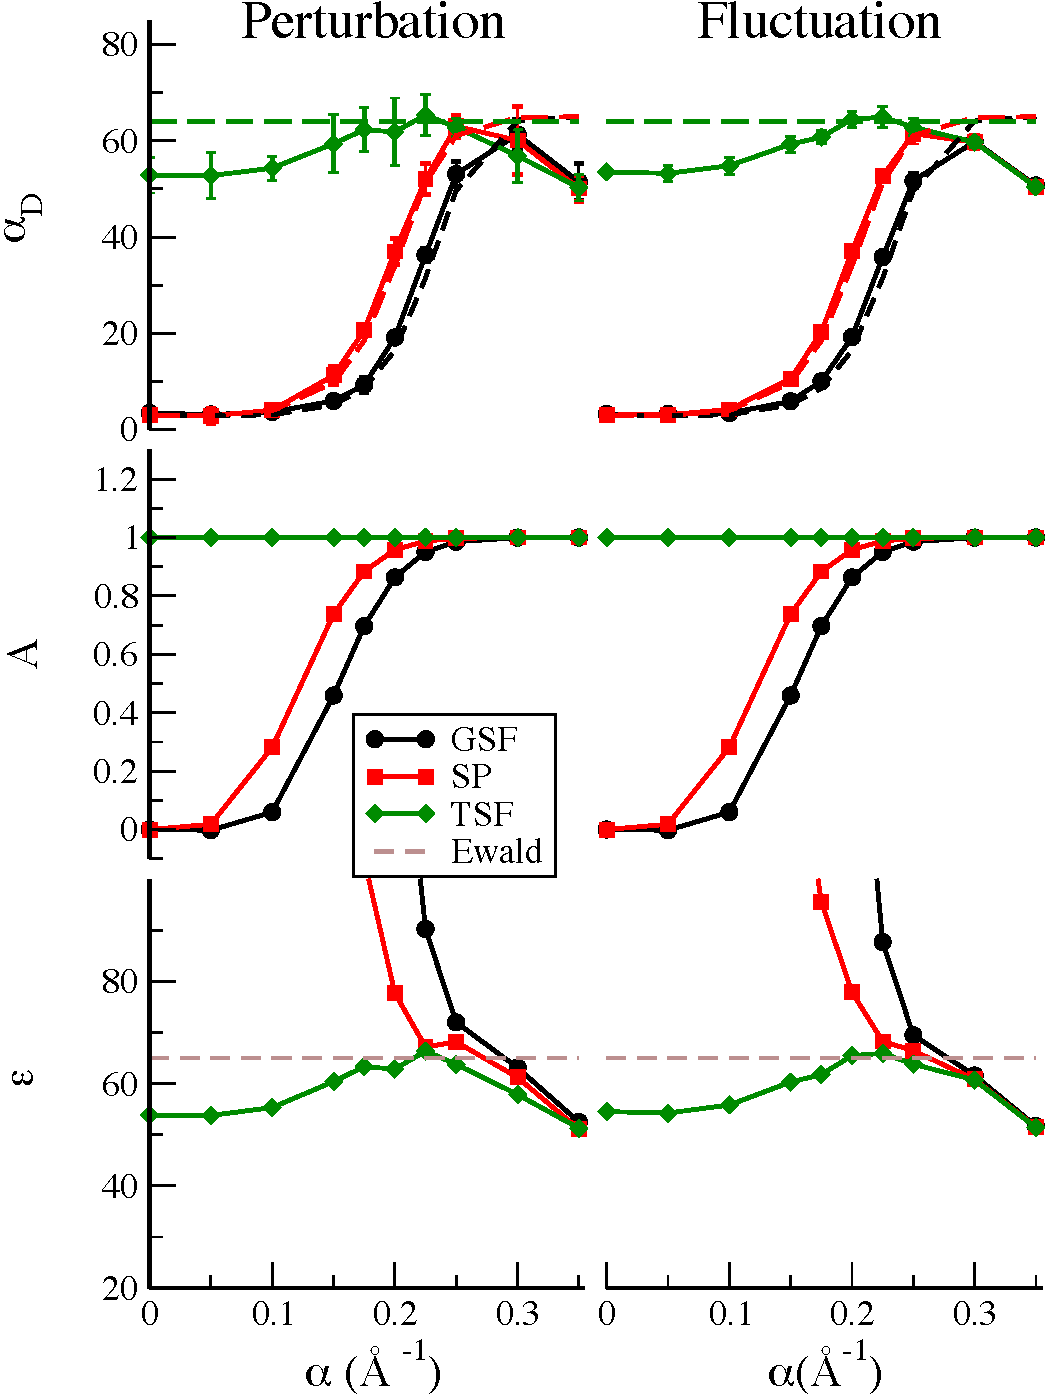
\includegraphics[width=4.5in]{dielectricFinal_Dipole.pdf}
\caption{The polarizability ($\alpha_D$), correction factor ($A$), and
  dielectric constant ($\epsilon$) for the test dipolar fluid. The
  left panels were computed using external fields, and those on the
  right are the result of equilibrium fluctuations.  In the GSF and SP
  methods, the corrections are large in with small values of $\alpha$,
  and a optimal damping coefficient is evident around 0.25 \AA$^{-1}$.
  The dashed lines in the upper panel indicate back-calculation of the
  polarizability using the Ewald estimate (Refs.\cite{Adams81}
  and \cite{NeumannI83}) for the dielectric constant.}
\label{fig:dielectricDipole}
\end{center}
\end{figure}
The macroscopic polarizability ($\alpha_D$) for the dipolar fluid is
shown in the upper panels in Fig. \ref{fig:dielectricDipole}.  The
polarizability obtained from the both perturbation and fluctuation
approaches are in excellent agreement with each other.  The data also
show a stong dependence on the damping parameter for both the Shifted
Potential (SP) and Gradient Shifted force (GSF) methods, while Taylor
shifted force (TSF) is largely independent of the damping
parameter.

The calculated correction factors discussed in section
\ref{sec:corrFactor} are shown in the middle panels. Because the TSF
method has $A = 1$ for all values of the damping parameter, the
computed polarizabilities need no correction for the dielectric
calculation. The value of $A$ varies with the damping parameter in
both the SP and GSF methods, and inclusion of the correction yields
dielectric estimates (shown in the lower panel) that are generally too
large until the damping reaches $\sim$~0.25~\AA$^{-1}$. Above this
value, the dielectric constants are generally in good agreement with
previous simulation results.\cite{NeumannI83}

Fig.~\ref{fig:dielectricDipole} also contains back-calculations of
the polarizability using the reference (Ewald) simulation
results.\cite{NeumannI83} These are indicated with dashed lines in the
upper panels.  It is clear that the expected polarizability for the SP
and GSF methods are quite close to results obtained from the
simulations.  This indicates that the correction formula for the
dipolar fluid (Eq.~(\ref{correctionFormula})) is quite sensitive when
the value of $\mathrm{A}$ deviates significantly from unity.

These results also suggest an optimal value for the damping parameter
of ($\alpha \sim 0.2-0.3$~\AA$^{-1}$) when evaluating dielectric
constants of point dipolar fluids using either the perturbation and
fluctuation approaches for the new real-space methods.

\begin{figure}
\begin{center}
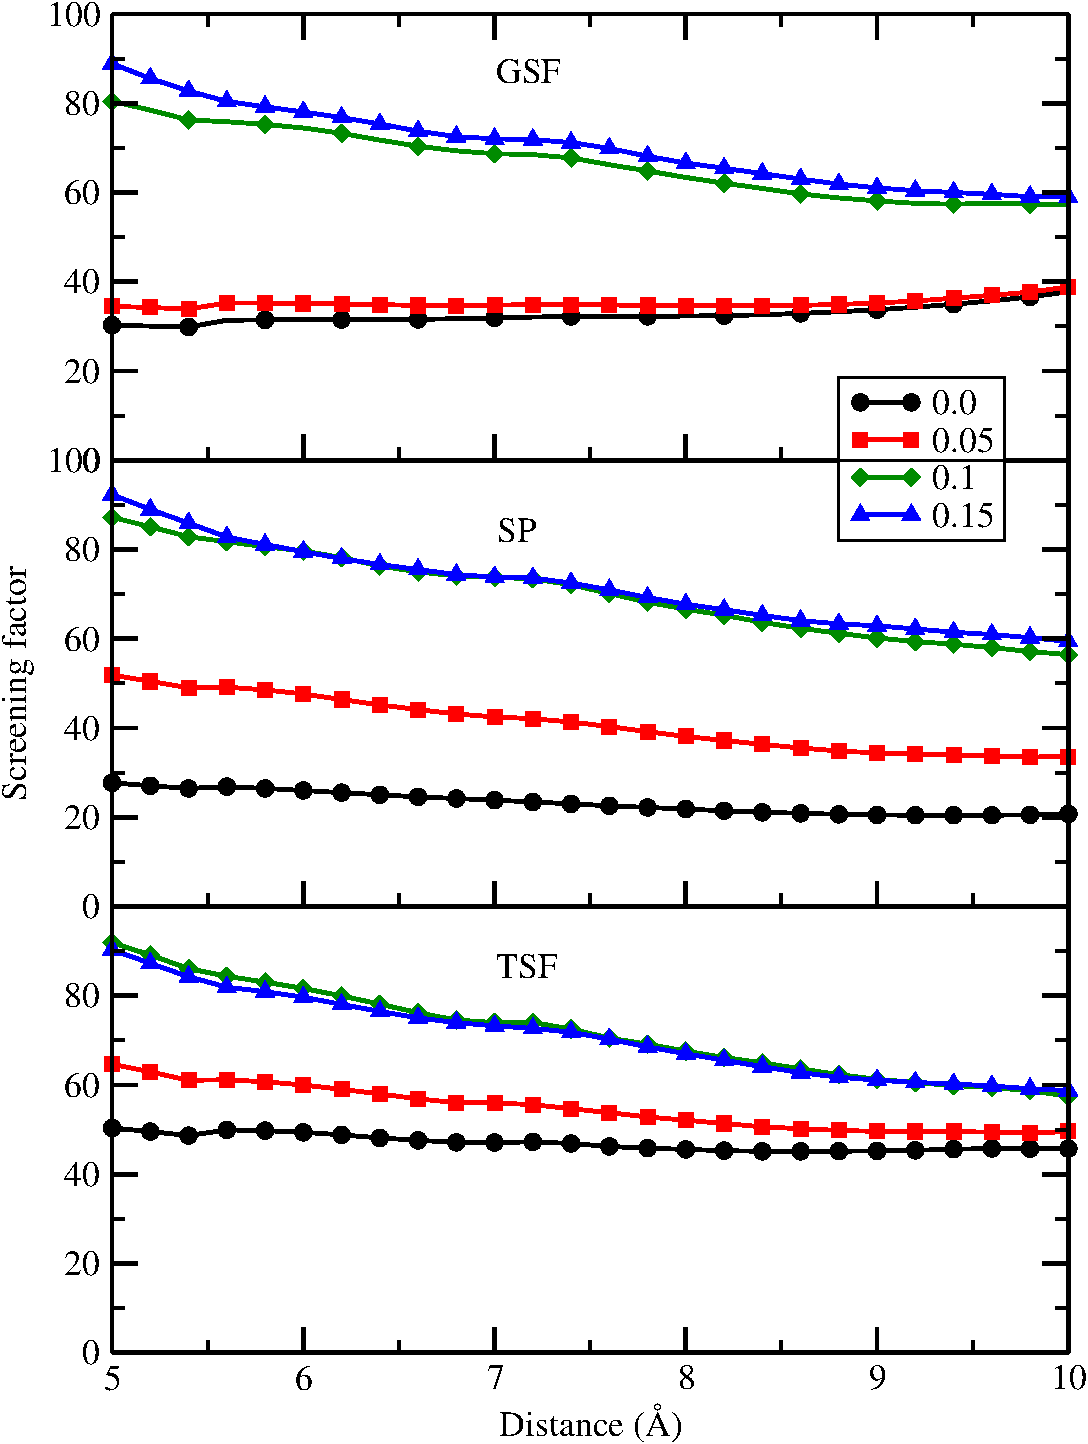
\includegraphics[width=4.5in]{ScreeningFactor_Dipole.pdf}
\caption{The distance-dependent screening factor, $\epsilon(r)$,
  between two ions immersed in the dipolar fluid. The new methods are
  shown in separate panels, and different values of the damping
  parameter ($\alpha$) are indicated with different symbols. All of
  the methods appear to be converging to the bulk dielectric constant
  ($\sim 65$) at large ion separations.}
\label{fig:ScreeningFactor_Dipole}
\end{center}
\end{figure}
We have also evaluated the distance-dependent screening factor,
$\epsilon(r)$, between two oppositely charged ions when they are
placed in the dipolar fluid.  These results were computed using
Eq.~(\ref{eq:pmf}) and are shown in Fig.
\ref{fig:ScreeningFactor_Dipole}.

The screening factor is similar to the dielectric constant, but
measures a local property of the ions in the fluid and depends on both
ion-dipole and dipole-dipole interactions. These interactions depend
on the distance between ions as well as the electrostatic interaction
methods utilized in the simulations. The screening should converge to
the dielectric constant when the field due to ions is small. This
occurs when the ions are separated (or when the damping parameter is
large). In Fig. \ref{fig:ScreeningFactor_Dipole} we observe that for
the higher value of damping alpha \textit{i.e.}
$\alpha = 0.2$~\AA$^{-1}$ and $0.3$~\AA$^{-1}$ and large separation
between ions, the screening factor does indeed approach the correct
dielectric constant.

It is also notable that the TSF method again displays smaller
perturbations away from the correct dielectric screening behavior.  We
also observe that for TSF method yields high dielectric screening even
for lower values of $\alpha$. 

At short distances, the presence of the ions creates a strong local
field that acts to align nearby dipoles nearly perfectly in opposition
to the field from the ions.  This has the effect of increasing the
effective screening when the ions are brought close to one another.
This effect is present even in the full Ewald treatment, and indicates
that the local ordering behavior is being captured by all of the
moderately-damped real-space methods.

\subsection{Quadrupolar fluid}
\begin{figure}
\begin{center}
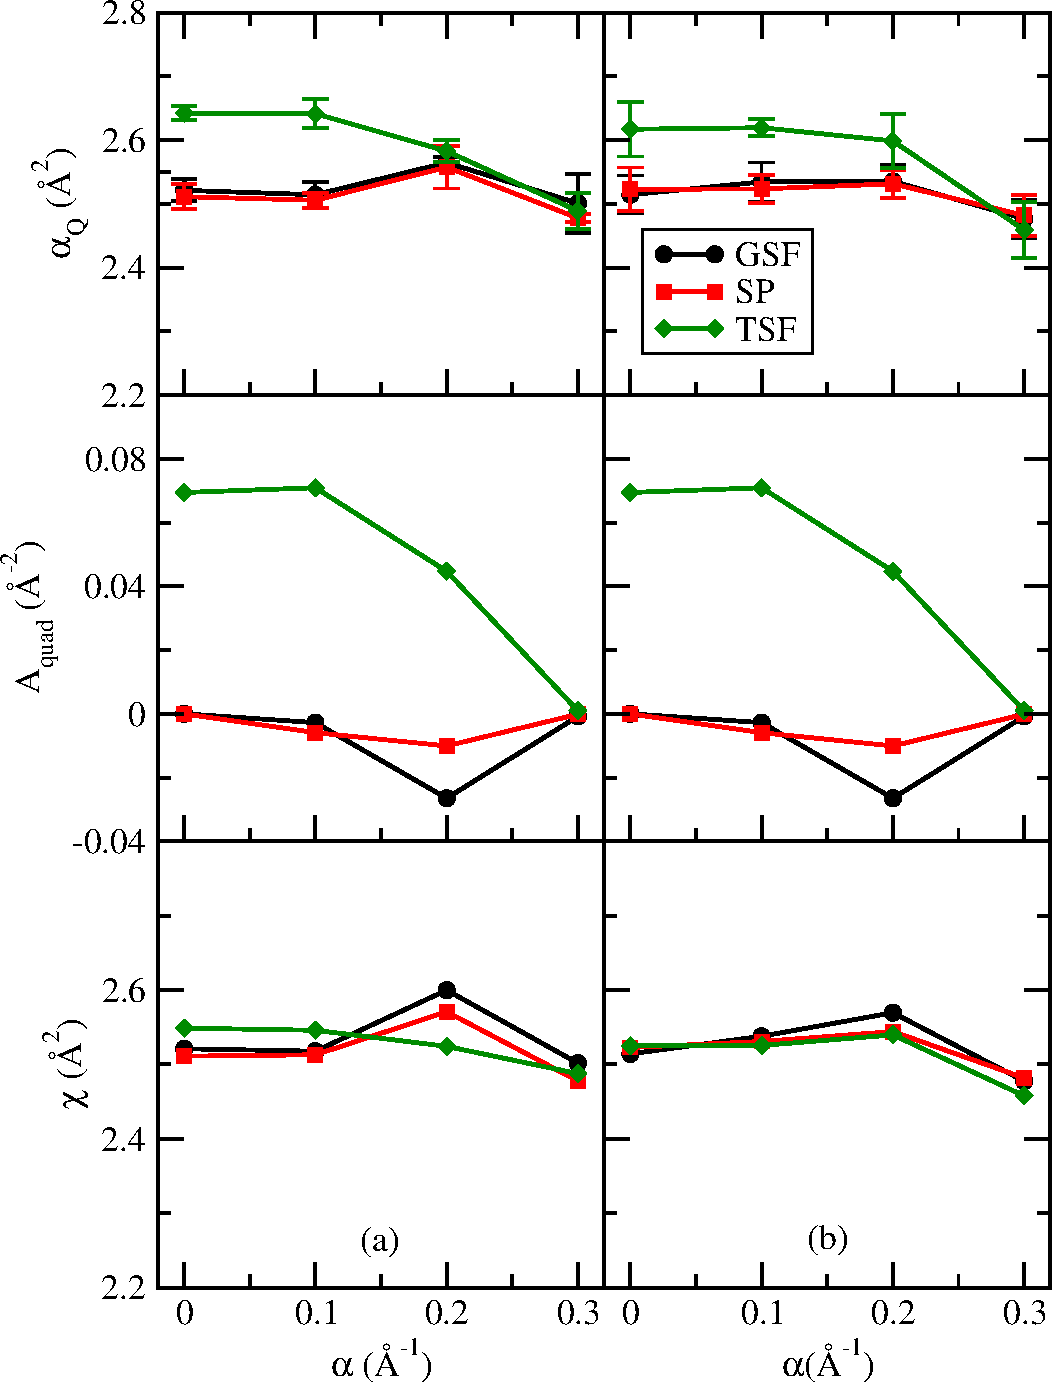
\includegraphics[width=4.5in]{polarizabilityFinal_Quad.pdf}
\caption{The quadrupole polarizability ($\alpha_Q$), correction factor
  ($B$), and susceptibility ($\chi_Q$) for the test quadrupolar
  fluid. The left panels were computed using external field gradients,
  and those on the right are the result of equilibrium fluctuations.
  The GSF and SP methods allow nearly unmodified use of the
  ``conducting boundary'' or polarizability results in place of the
  bulk susceptibility.}
\label{fig:dielectricQuad}
\end{center}
\end{figure}
The polarizability ($\alpha_Q$), correction factor ($B$), and
susceptibility ($\chi_Q$) for the quadrupolar fluid is plotted against
damping parameter Fig.  \ref{fig:dielectricQuad}.  In quadrupolar
fluids, both the polarizability and susceptibility have units of
$\mathrm{length}^2$. Although the susceptibility has dimensionality, it
is the relevant measure of macroscopic quadrupolar
properties.\cite{JeonI03, JeonII03} The left panel in
Fig. \ref{fig:dielectricQuad} shows results obtained from the applied
field gradient simulations whereas the results from the equilibrium
fluctuation formula are plotted in the right panels.

The susceptibility for the quadrupolar fluid is obtained from
quadrupolarizability and a correction factor using
Eq.~(\ref{eq:quadrupolarSusceptiblity}).  The susceptibilities are
shown in the bottom panels of Fig. \ref{fig:dielectricQuad}. All three
methods: (SP, GSF, and TSF) produce similar susceptibilities over the
range of damping parameters.  This shows that susceptibility derived
using the quadrupolarizability and the correction factors are
essentially independent of the electrostatic method utilized in the
simulation.

\begin{figure}
\begin{center}
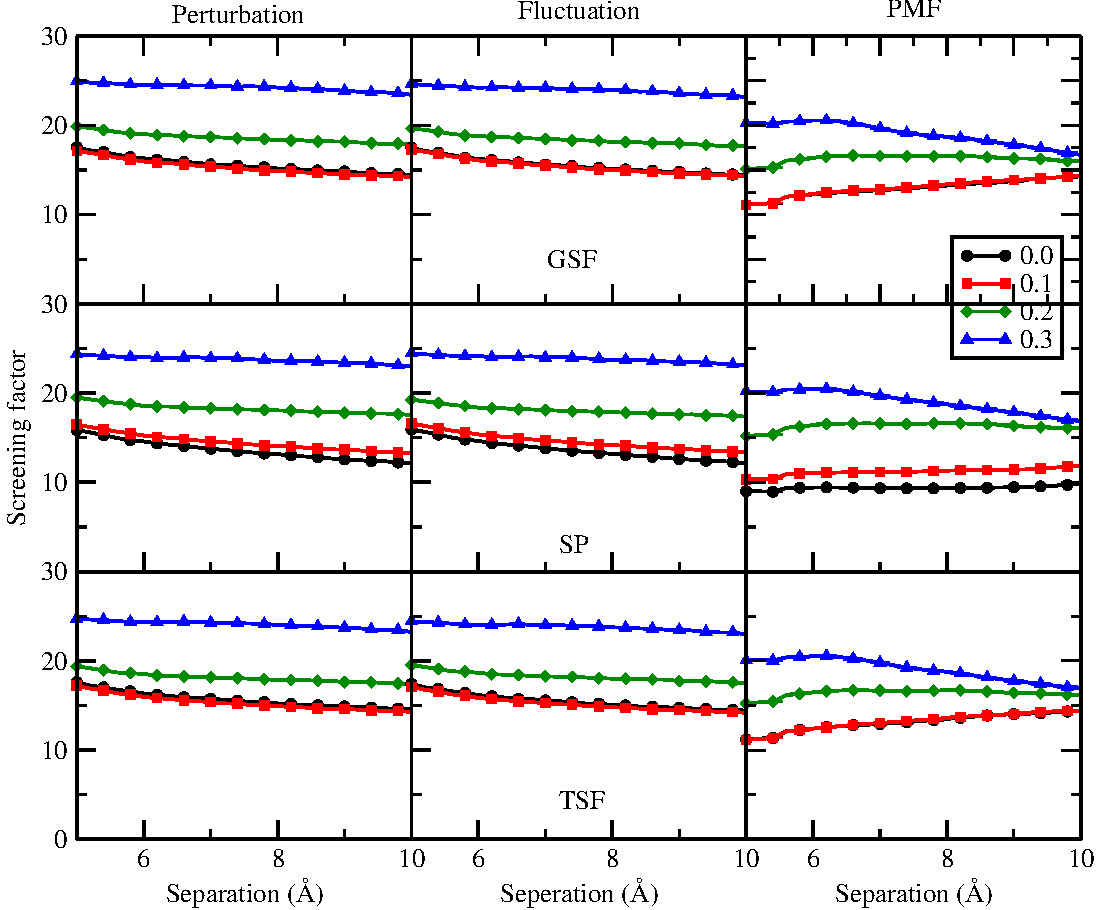
\includegraphics[width=\linewidth]{ScreeningFactor_Quad.pdf}
\caption{\label{fig:screenQuad} The distance-dependent screening
  factor, $\epsilon(r)$, between two ions immersed in the quadrupolar
  fluid. Results from  the perturbation and fluctuation methods are
  shown in right and central panels. Here the susceptibility is
  calculated from the  simulation and the geometrical factor is
  evaluated analytically, using the field and field-gradient produced
  by ions. The right hand panel shows the screening factor obtained
  from the PMF calculations.}
  \end{center}
\end{figure}
A more difficult test of the quadrupolar susceptibility is made by
comparing with direct calculation of the electrostatic screening using
the potential of mean force (PMF). Since the effective dielectric
constant for a quadrupolar fluid depends on the geometry of the field
and field gradient, this is not a physical property of the quadrupolar
fluid. 

The geometrical factor for embedded ions changes with the ion
separation distance. It is therefore reasonable to treat the
dielectric constant as a distance-dependent screening factor.  Since
the quadrupolar molecules couple with the gradient of the field, the
distribution of the quadrupoles will be inhomogeneously distributed
around the point charges.  Hence the distribution of quadrupolar
molecules should be taken into account when computing the geometrical
factors in the presence of this perturbation,
\begin{eqnarray}
G &=& \frac{\int_V g(\mathbf{r})  \left|\nabla \mathbf{E}^\circ
  \right|^2 d\mathbf{r}}{\int_V\left|\mathbf{E}^\circ\right|^2
  d\mathbf{r}}  \nonumber \\ \nonumber \\
 &=& \frac{ 2 \pi \int_{-1}^{1}  \int_{0}^{R} r^2  g(r,
     \cos\theta)  \left|\nabla \mathbf{E}^\circ  \right|^2 dr d(\cos\theta) }{\int_V\left|\mathbf{E}^\circ\right|^2 d\mathbf{r}}
\label{eq:geometricalFactor}
\end{eqnarray}
where $g(r,\cos\theta)$ is a distribution function for the quadrupoles
with respect to an origin at midpoint of a line joining the two probe
charges.

The effective screening factor is plotted against ion separation
distance in Fig. \ref{fig:screenQuad}.  The screening evaluated from
the perturbation and fluctuation methods are shown in right and
central panels. Here the susceptibility is calculated from the
simulation and the geometrical factor is evaluated analytically, using
the field and field-gradient produced by ions. The right hand panel
shows the screening factor obtained from the PMF calculations.

We note that the screening factor obtained from both the perturbation
and fluctuation formula show good agreement with the screening factor
calculated using PMF method. As there are no large differences in
quadrupole-quadruople interactions for various real-space
methods,\cite{PaperI,PaperII} we generally good agreement for the
screening factors using any of the real space methods.

\section{Summary}
We have used both perturbation and fluctuation approaches to evaluate
dielectric properties for dipolar and quadrupolar fluids.  The static
dielectric constant is the relevant bulk property for dipolar fluids,
while the quadrupolar susceptibility plays a similar role for
quadrupoles.  Corrections to both the static dielectric constant and
the quadrupolar susceptibility were derived for three new real space
electrostatic methods, and these corrections were tested against a
third measure of dielectric screening, the potential of mean force
between two ions immersed in the fluids.

For the dipolar fluids, we find that the polarizability evaluated
using the perturbation and fluctuation methods show excellent
agreement, indicating that equilibrium calculations of the dipole
fluctuations are good measures of bulk polarizability. One of the
findings of the Chapter 3 is that the moderately
damped GSF and SP methods were most suitable for molecular dynamics
and Monte Carlo simulations, respectively.\cite{PaperII}

The dielectric constant evaluated using the computed polarizability
and correction factors agrees well with the previous Ewald-based
simulation results \cite{Adams81,NeumannI83} for moderate damping
parameters in the range 0.25-0.3~\AA~$^{-1}$. 

Although the TSF method alters many dynamic and structural features in
multipolar liquids,\cite{PaperII} it is surprisingly good at computing
bulk dielectric properties at nearly all ranges of the damping
parameter.  In fact, the correction factor, $A = 1$, for the TSF
method so the conducting boundary formula is essentially correct when
using this method for point dipolar fluids.

The dielectric correction formula (Eq.~(\ref{correctionFormula}))
is extremely sensitive when the correction factor ($A$) deviates from
1, and this behavior is also seen in the effective screening of ions
embedded in the fluid. 

As in the dipolar case, the quadpole polarizability evaluated from
both perturbation and fluctuation simulations show excellent
agreement, again confirming that equilibrium fluctuation calculations
are sufficient to reproduce bulk dielectric properties in these
fluids.  The quadrupolar susceptibility calculated via our derived
correction factors tends to produce the same result for all three real
space methods.  Similarly, the screening factor calculated using the
susceptibility and a weighted geometric factor provides good agreement
with results obtained directly via potentials of mean force.  For
quadrupolar fluids, the distance dependence of the electrostatic
interaction is significantly reduced and the correction factors are
all small.  These points suggest that how an electrostatic method
treats the cutoff radius become less consequential for higher order
multipoles.
   
For this reason, we renew our recommendation that the
moderately-damped GSF method is an excellent choice for molecular
dynamics simulation where point-multipole interactions are being
utilized to compute bulk properties of fluids.

% % uncomment the following lines,
% if using chapter-wise bibliography
%
% \bibliographystyle{ndnatbib}
% \bibliography{example}
